\documentclass[11pt, oneside]{article}   	
\usepackage[top=1in, bottom=1.5in, left=1in, right=1in]{geometry}
\geometry{letterpaper}
\usepackage{graphicx}
\usepackage{amssymb, amsmath, enumerate}
\usepackage{caption,cancel}
\usepackage{subcaption}
\usepackage{booktabs,float,siunitx}
\usepackage{mathtools, hyperref}
\renewcommand{\vec}{\mathbf}
\renewcommand{\mod}{\text{ mod }}
\newcommand{\tr}{\text{tr }}
\renewcommand{\Re}{\text{Re}}
\renewcommand{\Im}{\text{Im}}
\DeclarePairedDelimiter\bra{\langle}{\rvert}
\DeclarePairedDelimiter\ket{\lvert}{\rangle}
\DeclarePairedDelimiterX\braket[2]{\langle}{\rangle}{#1 \delimsize\vert #2}
\newcommand{\kB}{k_\text{B}}
\newcommand{\ijnn}{{\langle{i,j}\rangle}}
\newcommand{\Tc}{T_\text{c}}
\newcommand{\Kc}{K_\text{c}}
  
\usepackage{color}
\usepackage{listings}
\usepackage{setspace}
\definecolor{Code}{rgb}{0,0,0}
\definecolor{Decorators}{rgb}{0.5,0.5,0.5}
\definecolor{Numbers}{rgb}{0.5,0,0}
\definecolor{MatchingBrackets}{rgb}{0.25,0.5,0.5}
\definecolor{Keywords}{rgb}{0,0,1}
\definecolor{self}{rgb}{0,0,0}
\definecolor{Strings}{rgb}{0,0.63,0}
\definecolor{Comments}{rgb}{0,0.63,1}
\definecolor{Backquotes}{rgb}{0,0,0}
\definecolor{Classname}{rgb}{0,0,0}
\definecolor{FunctionName}{rgb}{0,0,0}
\definecolor{Operators}{rgb}{0,0,0}
\definecolor{Background}{rgb}{0.98,0.98,0.98}
\lstdefinelanguage{Python}{
numbers=left,
numberstyle=\footnotesize,
numbersep=1em,
xleftmargin=1em,
framextopmargin=2em,
framexbottommargin=2em,
showspaces=false,
showtabs=false,
showstringspaces=false,
frame=l,
tabsize=4,
% Basic
basicstyle=\ttfamily\small\setstretch{1},
backgroundcolor=\color{Background},
% Comments
commentstyle=\color{Comments}\slshape,
% Strings
stringstyle=\color{Strings},
morecomment=[s][\color{Strings}]{"""}{"""},
morecomment=[s][\color{Strings}]{'''}{'''},
% keywords
morekeywords={import,from,class,def,for,while,if,is,in,elif,else,not,and,or,print,break,continue,return,True,False,None,access,as,,del,except,exec,finally,global,import,lambda,pass,print,raise,try,assert,format},
keywordstyle={\color{Keywords}\bfseries},
% additional keywords
morekeywords={[2]@invariant,pylab,numpy,np,scipy,plt,tnrange,matplotlib,pyplot,pickle,tqdm},
keywordstyle={[2]\color{Decorators}\slshape},
emph={self},
emphstyle={\color{self}\slshape},
%
}
\linespread{1.25}


\title{212: Final Project\\Cluster Monte Carlo on a square lattice in 2, 3, \& 5 dimensions}
\author{Logan Bishop-Van Horn}
\date{\today}

\begin{document}
\maketitle
%%%%%%%%%%%%%%%%%%%%%%%%%%%%%%%%%%%%%%%%%%%%%%%%%%%%
%
% Section: Introduction
%
%%%%%%%%%%%%%%%%%%%%%%%%%%%%%%%%%%%%%%%%%%%%%%%%%%%%
\section{Introduction}
%%%%%%%%%%%%%%%%%%%%%%%%%%%%%%%%%%%%%%%%%%%%%%%%%%%%
% Subsection: Ising Model
%%%%%%%%%%%%%%%%%%%%%%%%%%%%%%%%%%%%%%%%%%%%%%%%%%%%
\subsection{Ising Model}
The Ising Model, invented by Lenz in 1920 and solved in one dimension by his student Ising in 1924, is a model for ferromagnetism consisting of discrete variables known as spins lying on a lattice, each of which can take on the value $+1$ (`up') or $-1$ (`down'). The model can be parameterized by the interactions or couplings amongst spins, and the coupling between individuals spins and an external magnetic field. In the trivial case where the spins do not interact, the physics is identical to that of a single spin in a magnetic field. Explicitly, the energy of a single spin with magnetic dipole moment $\mu$ and spin $s=\pm1$ in a magnetic field $B$ is given by the Hamiltonian $H_\text{1 spin}=-\mu Bs$, with $H_\text{1 spin}\ket{s}=E_s\ket{s}$, where the minus sign comes in because the energy is minimized when $s$ and $B$ have the same sign. The partition function for this simple system at temperature $T$ is given by
$$Z_\text{1 spin} = \sum_{s=\pm1}e^{-\frac{E_s}{\kB T}}\equiv\sum_{s=\pm1}e^{-\beta E_s}=\sum_{s=\pm1}e^{\beta\mu Bs}=2\cosh h,$$
where $h\equiv\beta\mu B$ is a dimensionless measure of the strength of the magnetic interaction relative to the thermal energy of the system. The magnetization, or average value of the spin, for a given $h$ is
$$m_h\equiv\langle{s}\rangle_h=\frac1{Z_\text{1 spin}}\sum_{s=\pm1}se^{-\beta E_s}=\frac1{Z_\text{1 spin}}\sum_{s=\pm1}se^{hs}=\frac{e^{+h}-e^{-h}}{2\cosh h}=\tanh h.$$
In the case of a system of $N$ noninteracting spins, the partition function $Z_\text{$N$ spins}$ is simply $(Z_\text{1 spin})^N$, and the magnetization per spin is precisely what we've written above.

In the next simplest case, each spin interacts only with its nearest neighbors on the lattice, and there is a single coupling constant $J$ that characterizes the strength of these interactions. In this case, for a given spin configuration $\{s_i\}$, the total energy of the system is
$$E(\{s_i\})=-J\sum_\ijnn s_is_j-\mu B\sum_is_i,$$
where the notation $\ijnn$ indicates that indices $i$ and $j$ correspond to lattice nearest neighbors. The Ising partition function is then
$$Z=\sum_{\{s_i\}}e^{-\beta E(\{s_i\})}=\sum_{\{s_i\}}\exp\left[\beta J\sum_\ijnn s_is_j+\beta\mu B\sum_is_i\right]\equiv\sum_{\{s_i\}}\exp\left[K\sum_\ijnn s_is_j+h\sum_is_i\right],$$
where $K$ is dimensionless and characterizes the energy scale of the spin-spin interactions relative to the thermal energy of the system. Qualitatively, when $K\ll1$ (that is, when the interactions are much weaker than thermal fluctuations) one would expect the system to be disordered, and when $K\gg1$ (i.e. when the interactions are much stronger than thermal fluctuations) one would expect the system to be ordered.

In one dimension, as Ising himself showed, the model hosts no phase transitions. However, the two-dimensional Ising model is one of the simplest models which does exhibit a phase transition. There are various approximation and expansion schemes dedicated to finding the critical coupling $\Kc$ (or critical temperature $\Tc\equiv1/K_c$, given in units of $J/\kB$) at which the system transitions from a disordered to an ordered state, as well as for finding the scaling of physical observables near criticality, which is dictated by the universality class of the model.

While at first glance the Ising model seems very amenable to numerical simulation, naive calculation of observables via direct enumeration of all possible spin configurations very quickly becomes computationally intractable beyond very small lattices in a very small number of dimensions. For numerical simulations of the Ising model to be feasible, we need an efficient way of generating spin configurations $\{s_i\}$ in such a way that the configurations have the correct Boltzmann weights $e^{-\beta E(\{s_i\})}$.
%%%%%%%%%%%%%%%%%%%%%%%%%%%%%%%%%%%%%%%%%%%%%%%%%%%%
% Subsection: Monte Carlo Methods
%%%%%%%%%%%%%%%%%%%%%%%%%%%%%%%%%%%%%%%%%%%%%%%%%%%%
\subsection{Monte Carlo Methods}
Suppose the spin configurations are Boltzmann-distributed. That is, each spin configuration $\{s_i\}$ occurs with probability
$$P(\{s_i\})=\frac{e^{-\beta E(\{s_i\})}}{\sum_{\{s_i\}}e^{-\beta E(\{s_i\})}}=\frac1Ze^{-\beta E(\{s_i\})}.$$
If there are $N$ spins in the system, then there are $2^N$ possible spin configurations, and the expected value of an observable $\mathcal{O}$ is given by
$$\langle\mathcal{O}\rangle=\sum_{\{s_i\}}\mathcal{O}(\{s_i\})P(\{s_i\}).$$
The idea behind all Monte Carlo methods is to generate some sample of $M\ll2^N$ configurations $\{s_m\}$ such that for $N\gg1$ the expected value of the observable $\mathcal{O}$ can be approximated by the sample average of $\mathcal{O}$:
$$\langle\mathcal{O}\rangle\approx\frac1M\sum_m\mathcal{O}(\{s_m\}).$$
The most famous method for generating sample configurations is known as the Metropolis algorithm. Very briefly, the Metropolis algorithm for an Ising system goes as follows:
\begin{enumerate}
\item{Choose some initial spin configuration (e.g., set each spin to $+1$ or $-1$ with equal probability), with fixed system temperature $\beta$.}
\item{Make a trial change to the spin configuration (i.e., flip the sign of a randomly-chosen spin).}
\item{Compute the change in energy $\Delta E$ between the initial spin configuration and the configuration after the trial spin flip. If $\Delta E<0$, accept the trial flip with probability 1. If $\Delta E>0$, accept the trial flip with probability $w=e^{-\beta\Delta E}$.}
\item{Repeat step 3 many times until the system reaches thermal equilibrium.}
\item{Calculate averages of physical observables.}
\end{enumerate}
Unfortunately, near the critical coupling $\Kc$, algorithms such as Metropolis, which are based on flipping a single spin at a time and are therefore inherently local, suffer from so-called ``critical slowing down'' resulting from the scale-invariance of fluctuations near a critical point. This means that as one approaches the phase transition, such algorithms struggle to efficiently generate relevant spin configurations.
%%%%%%%%%%%%%%%%%%%%%%%%%%%%%%%%%%%%%%%%%%%%%%%%%%%%
% Subsection: Cluster Monte Carlo
%%%%%%%%%%%%%%%%%%%%%%%%%%%%%%%%%%%%%%%%%%%%%%%%%%%%
\subsection{Cluster Monte Carlo}
To avoid the problems created by critical slowing down, so-called Cluster Monte Carlo were developed, in which instead of flipping a single spin at a time, large clusters of spins are flipped simultaneously with a high probability.
%%%%%%%%%%%%%%%%%%%%%%%%%%%%%%%%%%%%%%%%%%%%%%%%%%%%
% Subsubsection: SW Algorithm
%%%%%%%%%%%%%%%%%%%%%%%%%%%%%%%%%%%%%%%%%%%%%%%%%%%%
\subsubsection{Swendsen-Wang Algorithm}
One of the original cluster Monte Carlo algorithms was developed by Swendsen and Wang in 1987 [Phys. Rev. Lett., 58 (2): 86 (1987).]. To construct the clusters that will later be flipped, we introduce a bond index $b$ connecting two interacting spins $s_{i(b)}s_{j(b)}$, where $b=1,2,\ldots,dN$ for a $d$ dimensional cubic lattice with $N$ sites. The total energy of a given spin configuration $\{s_i\}$ is then
$$E(\{s_i\})=-|J|\sum_{b=1}^{dN}[1+s_{i(b)}s_{j(b)}]=\sum_{b=1}^{dN}E_b.$$
The gives us the following partition function:
$$Z=\sum_{\{s_i\}}e^{-\beta E(s_i\})}=\sum_{\{s_i\}}e^{\beta E_b}=\sum_{\{s_i\}}\prod_{b=1}^{dN}[1+(e^{\beta E_b}-1)]\equiv\sum_{\{s_i\}}\prod_{b=1}^{dN}[F_b(0)+F_b(1)],$$
for a bond function $F_b$ defined on $\{0,1\}$ as
$$F_b(s)=\begin{cases}
1&\text{for $s=0$}\\
e^{\beta E_b}-1&\text{for $s=1$}
\end{cases}.$$
Note that the bond function $F_b$ depends on the value of the spins $s_{i(b)}$, $s_{j(b)}$ connected by bond $b$:
\begin{align*}
F_b(0)=&1\,\forall s_{i(b)}, s_{j(b)}\\
F_b(1)=&\begin{cases}
	e^{2\beta|J|}-1&\text{for $s_{i(b)}=s_{j(b)}$}\\
	0&\text{for $s_{i(b)}\neq s_{j(b)}$}
\end{cases}
\end{align*}
For each bond $b$, we can define a bond variable $\tau_b=\pm1$, allowing us to rewrite the partition function as a sum over spin configurations $\{s_i\}$ and bond configurations $\{\tau_b\}$:
$$Z=\sum_{\{s_i\}}\sum_{\{\tau_b\}}\prod_{b=1}^{dN}F_b(\tau_b).$$
A bond with $\tau_b=1$ corresponds to a bond between parallel spins, and is known as a filled bond. We can see that the probability weight for a given spin and bond configuration is
$$W(\{s_i\}, \{\tau_b\})=\prod_{b=1}^{dN}F_b(\tau_b)=(e^{2\beta|J|}-1)^{N_f},$$
where $N_f$ is the number of filled bonds on the lattice. For a given spin configuration, the probability of bond configuration $\{\tau_b\}$ is
$$P(\{\tau_b\})=\prod_{b=1}^{dN}P_b(\tau_b),\text{ where }P_b(\tau_b)=\frac{F_b(\tau_b)}{F_b(0)+F_b(1)}.$$
Therefore the probability associated with a filled bond $\tau_b=1$ is
$$P_b(\tau_b=1)=\begin{cases}
	1-e^{2\beta|J|}&\text{for $s_{i(b)}=s_{j(b)}$}\\
	0&\text{for $s_{i(b)}\neq s_{j(b)}$}
\end{cases}$$
Note that for a given spin and bond configuration, if we simultaneously flip all spins in a cluster connected by filled bonds, the weight $W(\{s_i\}, \{\tau_b\})=(e^{2\beta|J|}-1)^{N_f}$ is unchanged. With this observation, we can define a single Monte Carlo step of the Swendsen-Wang algorithm as follows:
\begin{enumerate}
	\item{Start with a random configuration of spins}
	\item{Populate filled bonds between spins $s_{i(b)}$, $s_{j(b)}$ according to the probabilities
	$$P_b(\tau_b=1)=\begin{cases}
	1-e^{2\beta|J|}&\text{for $s_{i(b)}=s_{j(b)}$}\\
	0&\text{for $s_{i(b)}\neq s_{j(b)}$}
\end{cases}$$}
	\item{Flip all resulting clusters of spins with probability $1/2$}
\end{enumerate}
%%%%%%%%%%%%%%%%%%%%%%%%%%%%%%%%%%%%%%%%%%%%%%%%%%%%
% Subsubsection: Wolff Algorithm
%%%%%%%%%%%%%%%%%%%%%%%%%%%%%%%%%%%%%%%%%%%%%%%%%%%%
\subsubsection{Wolff Algorithm}
A somewhat simpler cluster Monte Carlo algorithm was published in 1989 by Wolff [Phys. Rev. Lett., 62 (4): 361 (1989).]. In the Wolff algorithm, a single spin cluster is constructed at each Monte Carlo step and flipped with probability 1. A single Monte Carlo step of the Wolff algorithm goes as follows:
\begin{enumerate}
	\item{Start with a random spin configuration}
	\item{Select a lattice site $i$ at random. This site will be the ``seed'' of the cluster}
	\item{For each of $i$'s nearest neighbors $j$, if $i$ and $j$ are parallel and the bond between $i$ and $j$ has not already been counted, add $j$ to the cluster with probability $1-e^{-2\beta J}$ }
	\item{Place each spin $j$ that gets added to the cluster onto the stack. After all of $i$'s neighbors have been considered, repeat step 2 with the site $j$ that is on the top of the stack. Repeat until the stack is empty}
	\item{Finally, flip all spins in the cluster.}
\end{enumerate}
%%%%%%%%%%%%%%%%%%%%%%%%%%%%%%%%%%%%%%%%%%%%%%%%%%%%
%
% Section: Implementation
%
%%%%%%%%%%%%%%%%%%%%%%%%%%%%%%%%%%%%%%%%%%%%%%%%%%%%
\section{Implementation}
I've written a small Python module that performs temperature sweeps of a zero-field Ising system with nearest neighbor interactions on a cubic lattice in any integer number of dimensions using the Wolff algorithm, and calculates physical observables such as magnetization, susceptibility, specific heat, and spin-spin correlation at each temperature. The program consists of three classes: \lstinline[language=Python]{Lattice}, \lstinline[language=Python]{Ising}, and \lstinline[language=Python]{IsingTempSeries}.
\begin{itemize}
\item{\lstinline[language=Python]{Lattice} class: Defines a cubic lattice with a given linear size, in a given dimension, and at a given temperature (in units of $J/\kB$). Includes methods for generating a random spin configuration, selecting a spin at random, finding nearest neighbors (with periodic boundary conditions), building clusters according to the Wolff algorithm, etc.}
\item{\lstinline[language=Python]{Ising} class: performs $N_\text{eq}$ ``equilibration'' iterations of the Wolff algorithm ($N_\text{eq}=10^4$ by default, but this is probably overkill) on a \lstinline[language=Python]{Lattice} at a given temperature, followed by $N_\text{eq}/2$ ``measurement'' iterations. Calculates magnetization per spin, susceptibility, and specific heat, Binder ratios, and spin-spin correlation averaged over all measurement iterations.}
\item{\lstinline[language=Python]{IsingTempSeries} class: Simulates an \lstinline[language=Python]{Ising} object for a given set of temperatures. Records and plots observables and diagnostics as a function of temperature.}
\end{itemize}
See Appendix A for a listing of the code, which is intended to be run inside a \href{http://jupyter-notebook-beginner-guide.readthedocs.io/en/latest/what_is_jupyter.html}{Jupyter Notebook} but could be easily modified to run from a terminal. 
%An example notebook is available on \href{}{GitHub}.
To simulate, for example, a $20\times20$ lattice at $50$ temperatures from $J/\kB$ to $4J/\kB$, one could run the following commands in a Jupyter Notebook (assuming the module is defined in \lstinline[language=Python]{ising.py} and is in the Python path):
\begin{lstlisting}[language=Python]
from ising import *
%matplotlib inline

ising_20_2_50 = IsingTempSeries(20, 2, 1, 4, 50)
ising_20_2_50.do_series()
ising_20_2_50.save('ising_20_2_50')
\end{lstlisting}
(Note: The cluster-building portion of the code is written in a recursive fashion. For large lattices or in many dimensions, you may hit the system recursion depth limit. There are ways around this issue, but for this project I was limited by computation time, not recursion depth. Systems up to about $N=10^3$ total lattice sites can simulated on a reasonable timescale on an old MacBook Pro.)
%%%%%%%%%%%%%%%%%%%%%%%%%%%%%%%%%%%%%%%%%%%%%%%%%%%%
%
% Section: Results
%
%%%%%%%%%%%%%%%%%%%%%%%%%%%%%%%%%%%%%%%%%%%%%%%%%%%%
\section{Results}
I will report the following physical observables/diagnostics, using $\langle{x}\rangle$ to denote the average of quantity $x$ over the $N_\text{eq}/2$ measurement iterations:
\begin{itemize}
	\item{Magnetization: $\langle{m}\rangle\equiv\langle\frac1{N}\sum_is_i\rangle$.}
	\item{Susceptibility: $\chi\equiv\frac{N}{T}(\langle{m^2}\rangle-\langle{m}\rangle^2)$.}
	\item{Specific heat: $C\equiv\frac{1}{T^2}(\langle{\epsilon^2}\rangle-\langle{\epsilon}\rangle^2),$ where $\epsilon$ is the energy per spin for a given spin configuration}
	\item{Spin-spin correlation function: $\langle{s_0s_r}\rangle-\langle{m}\rangle^2$}
	\item{First Binder ratio $Q\equiv Q_2=\frac{\langle{M^2}\rangle}{\langle{|M|}\rangle^2}$, where $M$ is the total magnetization of a given configuration. At low temperatures, $Q\to0$, at high temperatures, $Q\to\pi/2$, and the point at which $Q$ ratios from different lattices sizes are equal provides an accurate estimate for $T_\text{c}$.}
\end{itemize}
The critical exponents for two, three, and five dimensions are given in Table~\ref{tab:crit}.
\begin{table}[H]
\centering
\caption{Critical exponents for the cubic Ising model.}
\label{tab:crit}
\begin{tabular}{|c|c|c|c|}
\hline
 & $d=2$ & $d=3$ & $d=5$ \\ \hline
$\alpha$  & 0              & 0.11008(1)     & -1             \\ \hline
$\beta$   & 1/8            & 0.326419(3)    & 1/3            \\ \hline
$\gamma$  & 7/4            & 1.237075(10)   & 1              \\ \hline
$\eta$     & 1/4            & 0.036298(2)    & -1             \\ \hline
$\nu$     & 1              & 0.629971(4)    & 1/3            \\ \hline
\end{tabular}
\end{table}
%%%%%%%%%%%%%%%%%%%%%%%%%%%%%%%%%%%%%%%%%%%%%%%%%%%%
% Subsection: 2D
%%%%%%%%%%%%%%%%%%%%%%%%%%%%%%%%%%%%%%%%%%%%%%%%%%%%
\subsection{Two Dimensions}
In two dimensions, I simulated lattices with linear size $L=4,\,6,\,8,\,12,\,\&\,20$ at 50 temperatures from 1 to 4 (in units of $J/\kB$), and lattices with linear size $L=32,\&\,40$ at 15 temperatures from 2 to 3. Note that the two dimensional Ising model on a square lattice is exactly solvable, and the critical temperature is $T_\text{c, 2D}=2/\log(1+\sqrt2)\approx2.2691853$. Figure~\ref{fig:2D_all} shows observables and diagnostics resulting from $N_\text{eq}=10^4$ thermal equilibration Monte Carlo steps and $N_\text{eq}/2$ measurement steps. As expected, we see peaks in the susceptibility and specific heat near $T_\text{c, 2D}$, and the Binder ratios for different lattice sizes all intersect very close to $T_\text{c, 2D}$.

\begin{figure}
\begin{minipage}{0.47\textwidth}
    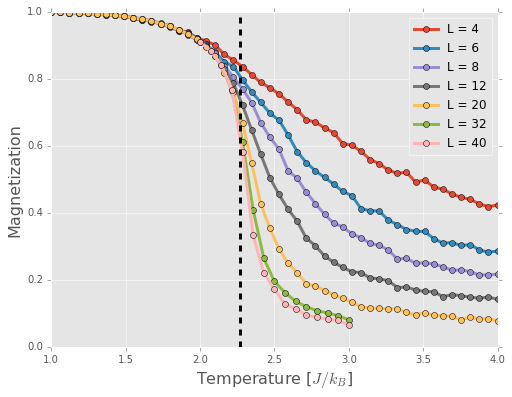
\includegraphics[width=\linewidth]{img/2D/mag}
    \end{minipage}
    \hspace{\fill} % note: no blank line here
    \begin{minipage}{0.47\textwidth}
    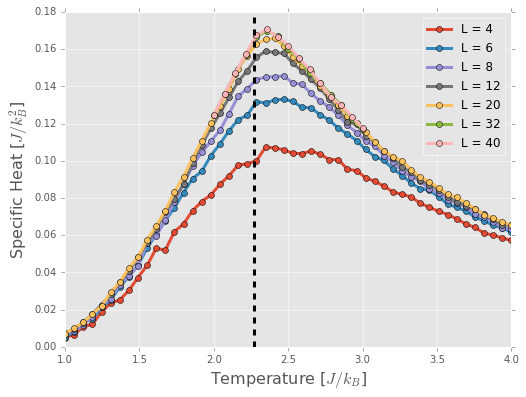
\includegraphics[width=\linewidth]{img/2D/C}
    \end{minipage}
    
    \vspace*{0cm} % vertical separation

    \begin{minipage}{0.47\textwidth}
    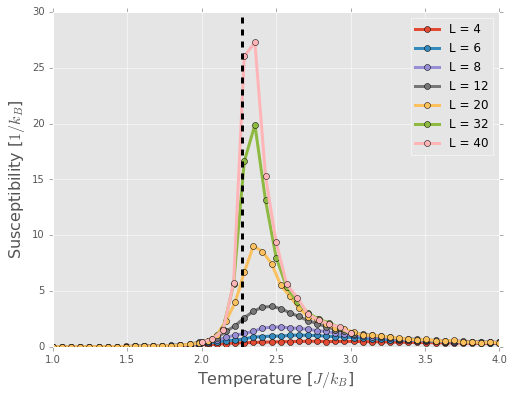
\includegraphics[width=\linewidth]{img/2D/susc_lin}
    \end{minipage}
    \hspace{\fill} % note: no blank line here
    \begin{minipage}{0.47\textwidth}
    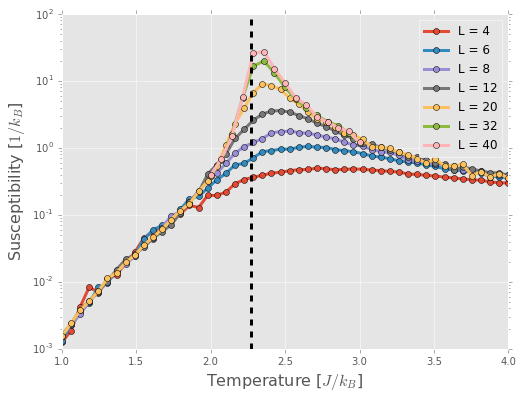
\includegraphics[width=\linewidth]{img/2D/susc}
    \end{minipage}

    \vspace*{0cm} % vertical separation

    \begin{minipage}{0.47\textwidth}
    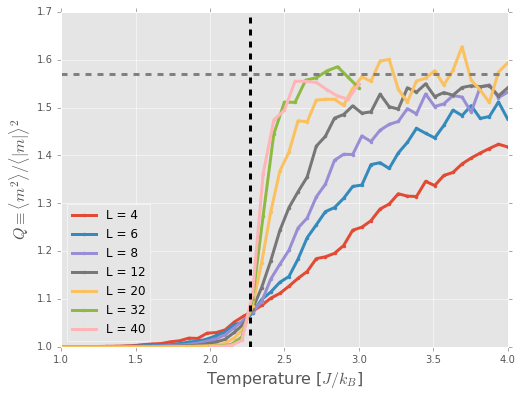
\includegraphics[width=\linewidth]{img/2D/binderQ}
    \end{minipage}
    \hspace{\fill} % note: no blank line here
    \begin{minipage}{0.47\textwidth}
    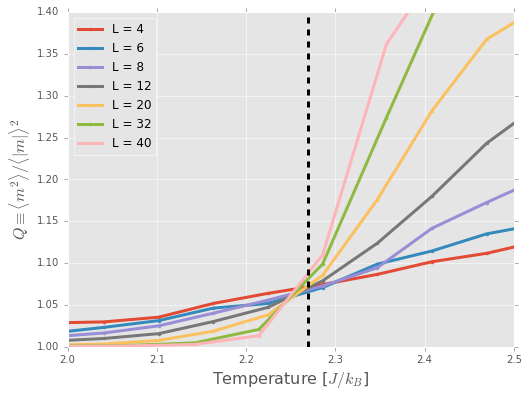
\includegraphics[width=\linewidth]{img/2D/binderQ_close}
    \end{minipage}
\caption{Two dimensions. Top row: Magnetization per spin (left) and specific heat (right). Middle row: susceptibility on linear (left) and semi-log (right) scales. Bottom row: Binder ratio $Q$ for the whole temperature sweep (left) and near $T_\text{c}$ (right). Dashed vertical line indicates exact critical temperature $T_{\text{c, 2D}}=2/\log(1+\sqrt2)$. Dashed horizontal line in the Binder ratio figure indicates theoretical high-temperature limit of $Q=\pi/2$.}
\label{fig:2D_all}
\end{figure}
Figure~\ref{fig:2D_corr} shows the spin-spin correlation function $\langle{s_0s_r}\rangle-\langle{m}\rangle^2$ for various temperatures and lattice sizes, as well as a semi-log plot of the correlation length $\xi$ derived from a fit to $\langle{s_0s_r}\rangle-\langle{m}\rangle^2=e^{-r/\xi}$. As expected, there is peak in the correlation length near the critical temperature.
\begin{figure}
\begin{minipage}{0.47\textwidth}
    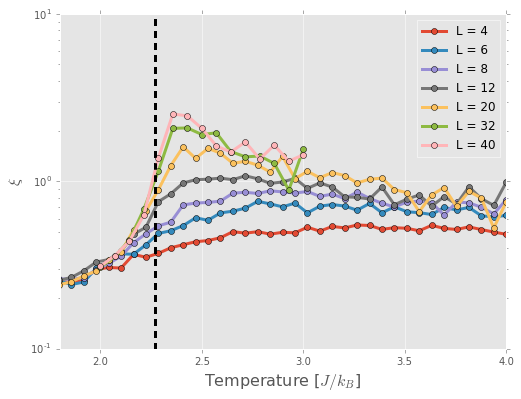
\includegraphics[width=\linewidth]{img/2D/xi_T}
    \end{minipage}
    \hspace{\fill} % note: no blank line here
    \begin{minipage}{0.47\textwidth}
    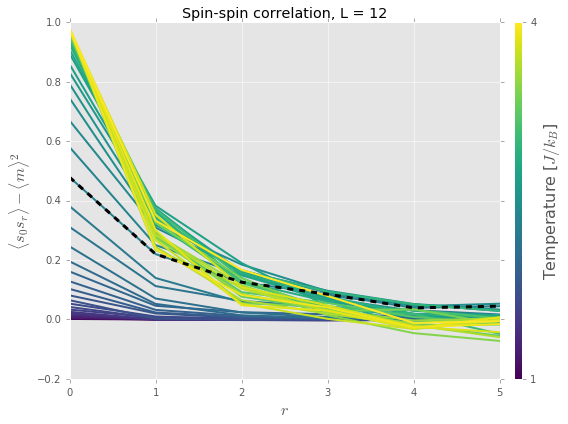
\includegraphics[width=\linewidth]{img/2D/spinspin12}
    \end{minipage}
    
    \vspace*{0cm} % vertical separation

    \begin{minipage}{0.47\textwidth}
    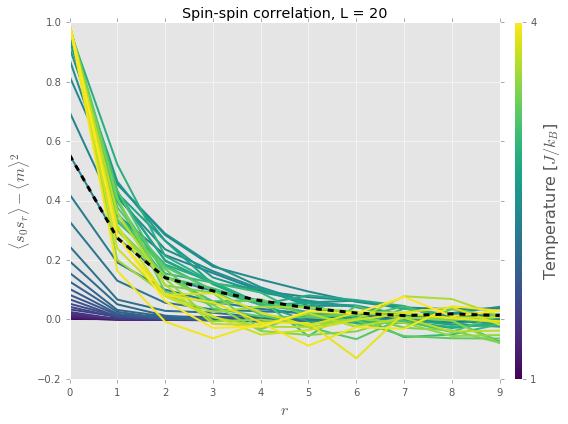
\includegraphics[width=\linewidth]{img/2D/spinspin20}
    \end{minipage}
    \hspace{\fill} % note: no blank line here
    \begin{minipage}{0.47\textwidth}
    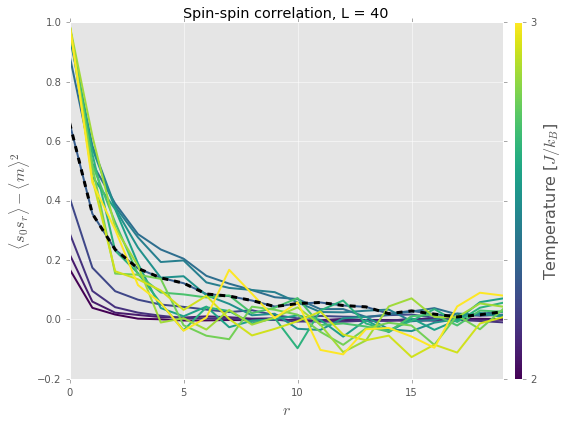
\includegraphics[width=\linewidth]{img/2D/spinspin40}
    \end{minipage}
\caption{Upper left: Semi-log plot of correlation length $\xi$ (extracted from a fit to an exponential $\propto e^{-r/\xi}$) as a function of temperature for various lattice sizes. Other panels: spin-spin correlation as a function of distance $r$ and temperature for $L=12,\,20,\,\&\,40$. Dotted line indicates temperature closest to $T_\text{c}$.}
\label{fig:2D_corr}
\end{figure}
Near $T_\text{c}$, the model has the following critical scaling behavior (with $t\equiv|T_\text{c}-T|/T_\text{c}$).
\begin{align*}
\langle{m}\rangle&\sim t^\beta\\
\chi&\sim t^{-\gamma}\\
C&\sim t^{-\alpha}\\
\xi&\sim t^{-\nu}\\
\langle{s_0s_r}\rangle-\langle{m}\rangle^2&\sim\frac{1}{r^{d-2+\eta}}\text{ at $T_\text{c}$}%\left(=e^{-\eta\log r}\text{ for $d=2$}\right),
\end{align*}
where $\chi$ is the susceptibility, $C$ is the specific heat, $\xi$ is the correlation length, $\langle{s_0s_r}\rangle$ is the spin-spin correlation function, and $d$ is the dimensionality of the system. Below $T_\text{c}$ we can fit the magnetization as a function of $T_\text{c}-T$ to a function of the form $A(T_\text{c}-T)^\beta$ with $A$ and $\beta$ free parameters. For the lattice sizes I considered, the magnetization clearly does not follow a power law, let alone one with the correct exponent (see Figure~\ref{fig:2D_mag_loglog}). A power law fit to the magnetization of the largest two-dimensional lattice ($L=40$) yields $\beta=0.10774231$, roughly 14\% smaller than the exact value of $\beta=1/8$. For smaller lattices, the observed $\beta$ is even smaller.
\begin{figure}[H]
   \centering
   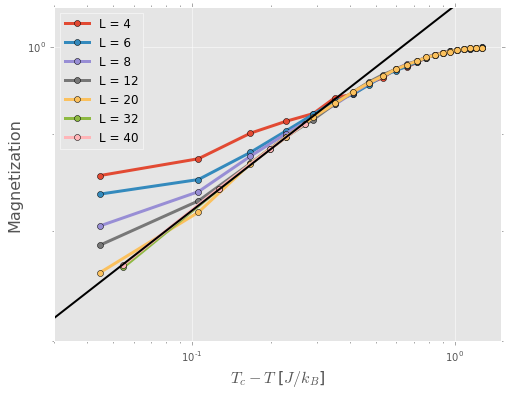
\includegraphics[width=0.6\textwidth]{img/2D/mag_loglog} % requires the graphicx package
   \caption{Log-log plot of the magnetization as a function of $T_\text{c}-T$ in two dimensions. Black line is a power law fit to the $L=40$ curve, yielding $\beta=0.10774231$.}
   \label{fig:2D_mag_loglog}
\end{figure}
We can apply finite size scaling techniques to estimate other critical exponents such as $\gamma$ and $\nu$. In particular, the maximum value of the susceptibility on a lattice of linear size $L$ should go as $\chi_\text{max}\sim L^{\gamma/\nu}$, and the reduced temperature at which the maximum occurs should go as $t_\text{max}\sim L^{-1/\nu}$. So we can estimate $\gamma$ and $\nu$ performing a power law fit on $\chi_\text{max}(L)$ and $t_\text{max}(L)$. In two dimensions, this procedure yields estimates of $\gamma/\nu\approx1.622$, $\nu\approx1.231$, $\gamma\approx1.997$. The exact values are $\nu=1$ and $\gamma=\gamma/\nu=7/4=1.75$. Figure~\ref{fig:2D_gam_nu} shows $\chi_\text{max}(L)$ and $t_\text{max}(L)$ on a log-log scale. We can see that $\chi_\text{max} (L)$ appears to follow a power law, but it seems that the point density near $T_\text{c}$ was not large enough to get an accurate $t_\text{max}$.
\begin{figure}[H]
   \centering
   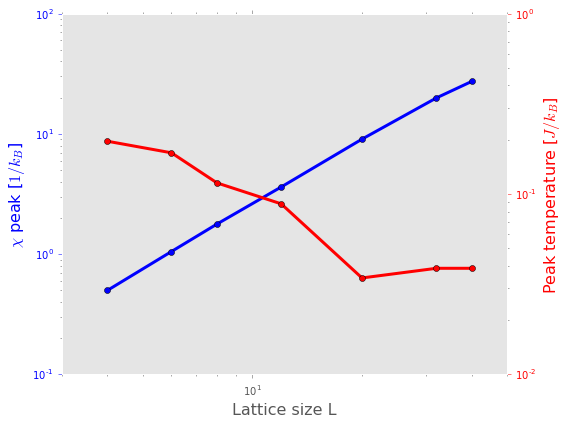
\includegraphics[width=0.6\textwidth]{img/2D/gam_nu} % requires the graphicx package
   \caption{Log-log plot of $\chi_\text{max}(L)$ and $t_\text{max}(L)$, yielding exponents of $\gamma/\nu\approx1.622$ and $\nu\approx1.231$.}
   \label{fig:2D_gam_nu}
\end{figure}
%%%%%%%%%%%%%%%%%%%%%%%%%%%%%%%%%%%%%%%%%%%%%%%%%%%%
% Subsection: 3D
%%%%%%%%%%%%%%%%%%%%%%%%%%%%%%%%%%%%%%%%%%%%%%%%%%%%
\subsection{Three Dimensions}
In three dimensions, I simulated lattices with linear size $L=3,\,4,\,6,\,\&\,8$ at 50 temperatures from 2 to 8, and lattices with linear size $L=10\,\&\,12$ at 15 temperatures from 3.5 to 5.5. I will be comparing to the published critical temperature of $T_{\text{c, 3D}}\approx1/0.2216544\approx4.511528$ [J. Phys. A 29: 5727-5734 (1996)]. Once again, we see peaks in the susceptibility and specific heat near $T_\text{c}$, and the Binder ratios meet very near to $T_\text{c}$.
\begin{figure}[H]
\begin{minipage}{0.47\textwidth}
    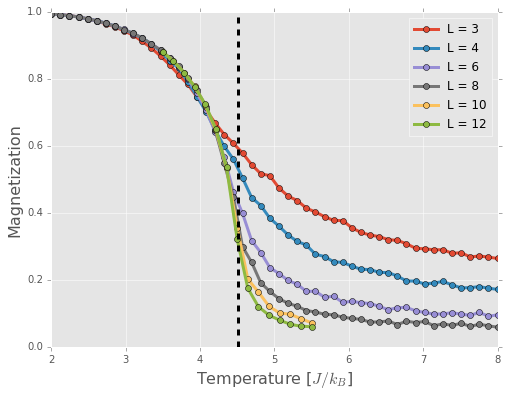
\includegraphics[width=\linewidth]{img/3D/mag}
    \end{minipage}
    \hspace{\fill} % note: no blank line here
    \begin{minipage}{0.47\textwidth}
    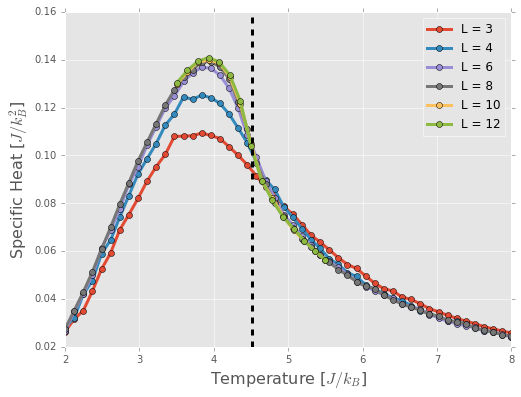
\includegraphics[width=\linewidth]{img/3D/C}
    \end{minipage}
    
    \vspace*{0cm} % vertical separation

    \begin{minipage}{0.47\textwidth}
    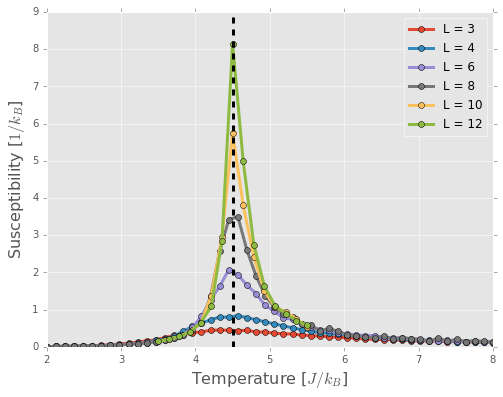
\includegraphics[width=\linewidth]{img/3D/susc_lin}
    \end{minipage}
    \hspace{\fill} % note: no blank line here
    \begin{minipage}{0.47\textwidth}
    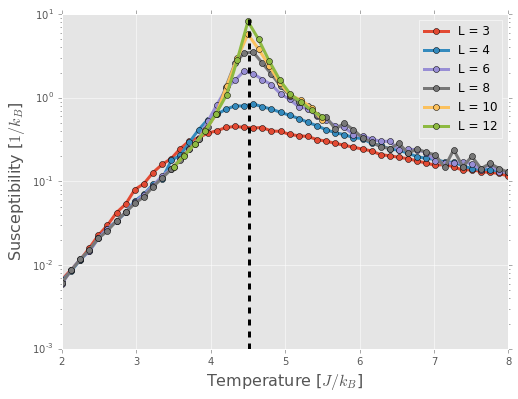
\includegraphics[width=\linewidth]{img/3D/susc}
    \end{minipage}

    \vspace*{0cm} % vertical separation

    \begin{minipage}{0.47\textwidth}
    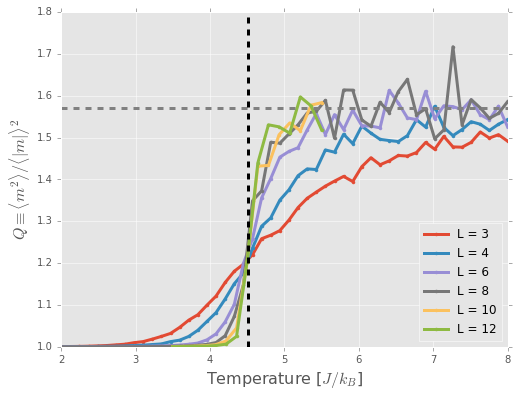
\includegraphics[width=\linewidth]{img/3D/binderQ}
    \end{minipage}
    \hspace{\fill} % note: no blank line here
    \begin{minipage}{0.47\textwidth}
    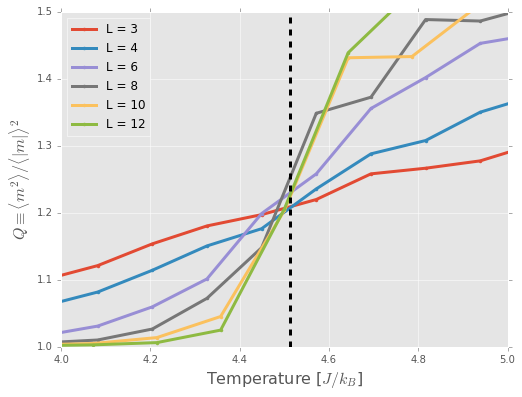
\includegraphics[width=\linewidth]{img/3D/binderQ_close}
    \end{minipage}
\caption{Three dimensions. Top row: Magnetization per spin (left) and specific heat (right). Middle row: susceptibility on linear (left) and semi-log (right) scales. Bottom row: Binder ratio $Q$ for the whole temperature sweep (left) and near $T_\text{c}$ (right). Dashed vertical line indicates critical temperature $T_{\text{c, 3D}}\approx1/0.2216544\approx4.511528$ [J. Phys. A 29: 5727-5734 (1996)]. Dashed horizontal line in the Binder ratio figure indicates theoretical high-temperature limit of $Q=\pi/2$.}
\label{fig:3D_all}
\end{figure}
Figure~\ref{fig:3D_corr} shows the spin-spin correlation function $\langle{s_0s_r}\rangle-\langle{m}\rangle^2$ for various temperatures and lattice sizes, as well as a semi-log plot of the correlation length $\xi$ derived from a fit to $\langle{s_0s_r}\rangle-\langle{m}\rangle^2=e^{-r/\xi}$. As expected, there is peak in the correlation length near the critical temperature.
\begin{figure}[H]
\begin{minipage}{0.47\textwidth}
    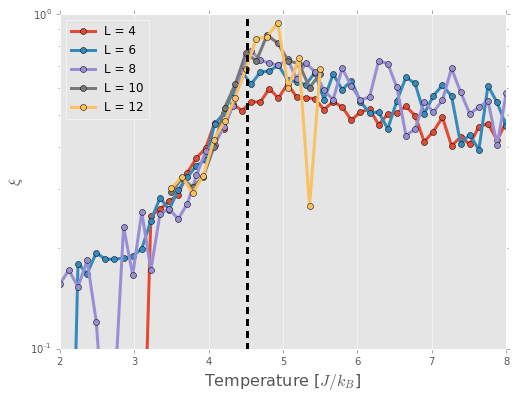
\includegraphics[width=\linewidth]{img/3D/xi_T}
    \end{minipage}
    \hspace{\fill} % note: no blank line here
    \begin{minipage}{0.47\textwidth}
    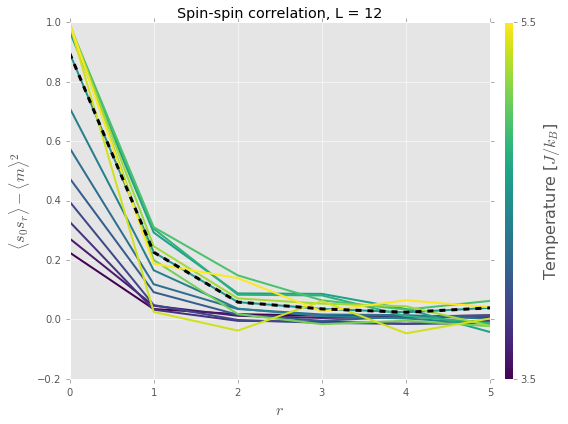
\includegraphics[width=\linewidth]{img/3D/spinspin12}
    \end{minipage}
\caption{Left: Semi-log plot of correlation length $\xi$ (extracted from a fit to an exponential $\sim e^{-r/\xi}$) as a function of temperature for various lattice sizes. Right: spin-spin correlation as a function of distance $r$ and temperature for $L=12$. Dotted line indicates temperature closest to $T_\text{c}$.}
\label{fig:3D_corr}
\end{figure}
Figure~\ref{fig:3D_mag_loglog} shows the magnetization as a function of temperature on a log-log scale, along with a power law fit to the $L=12$ data, yielding a best-fit of $\beta=0.23964831$, roughly 27\% below the literature value of $\beta=0.326419$ [J. Phys. A 29: 5727-5734 (1996)].
\begin{figure}[H]
   \centering
   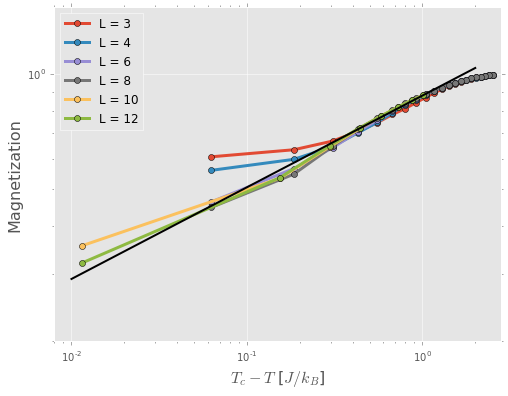
\includegraphics[width=0.6\textwidth]{img/3D/mag_loglog} % requires the graphicx package
   \caption{Log-log plot of the magnetization as a function of $T_\text{c}-T$ in three dimensions. Black line is a power law fit to the $L=12$ curve, yielding $\beta=0.23964831$.}
   \label{fig:3D_mag_loglog}
\end{figure}
Fitting $\chi_\text{max}(L)$ and $t_\text{max}(L)$ yields critical exponent estimates of $\gamma/\nu\approx2.033$, $\nu\approx0.547$, $\gamma\approx1.113$. The published values are $\nu=0.629971$ and $\gamma=1.237075$. This amounts to a $13\%$ error in $\nu$ and a $10\%$ error in $\gamma$. Once again the temperature point density near $T_\text{c}$ appears to be an issue in calculating $\nu$.
\begin{figure}[H]
   \centering
   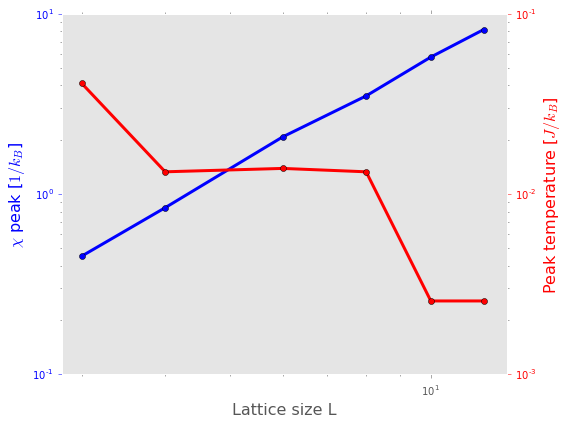
\includegraphics[width=0.6\textwidth]{img/3D/gam_nu} % requires the graphicx package
   \caption{Log-log plot of $\chi_\text{max}(L)$ and $t_\text{max}(L)$, yielding exponents of $\gamma/\nu\approx2.033$ and $\nu\approx0.547$.}
   \label{fig:3D_gam_nu}
\end{figure}
%%%%%%%%%%%%%%%%%%%%%%%%%%%%%%%%%%%%%%%%%%%%%%%%%%%%
% Subsection: 5D
%%%%%%%%%%%%%%%%%%%%%%%%%%%%%%%%%%%%%%%%%%%%%%%%%%%%
\subsection{Five Dimensions}
In five dimensions, I simulated lattices with linear size $L=2\,\&\,3$ at 50 temperatures from 2 to 12, and lattices with linear size $L=4\;(5)$ at 15 (10) temperatures from 8 to 9.5. I will be comparing to the published critical temperature of $T_{\text{c, 5D}}\approx1/0.11391498\approx8.7784767$ [Nuclear Physics B 895, 305-318 (2015)].
\begin{figure}[H]
\begin{minipage}{0.47\textwidth}
    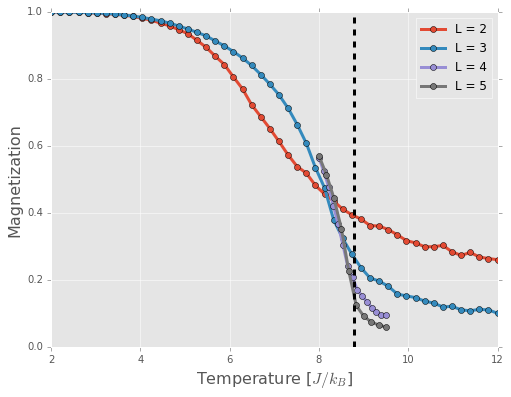
\includegraphics[width=\linewidth]{img/5D/mag}
    \end{minipage}
    \hspace{\fill} % note: no blank line here
    \begin{minipage}{0.47\textwidth}
    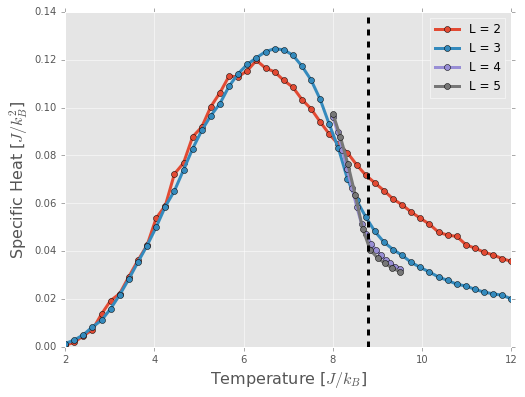
\includegraphics[width=\linewidth]{img/5D/C}
    \end{minipage}
    
    \vspace*{0cm} % vertical separation

    \begin{minipage}{0.47\textwidth}
    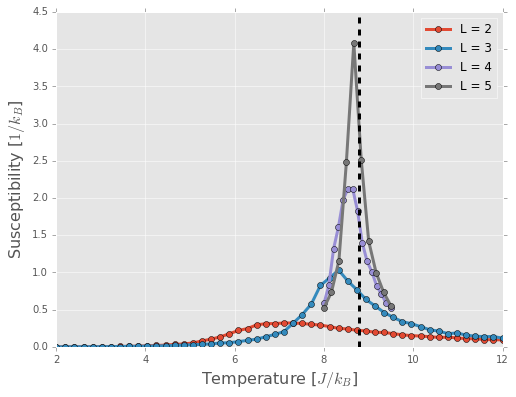
\includegraphics[width=\linewidth]{img/5D/susc_lin}
    \end{minipage}
    \hspace{\fill} % note: no blank line here
    \begin{minipage}{0.47\textwidth}
    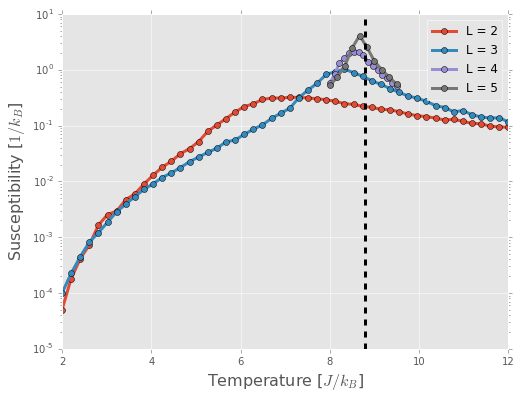
\includegraphics[width=\linewidth]{img/5D/susc}
    \end{minipage}

    \vspace*{0cm} % vertical separation

    \begin{minipage}{0.47\textwidth}
    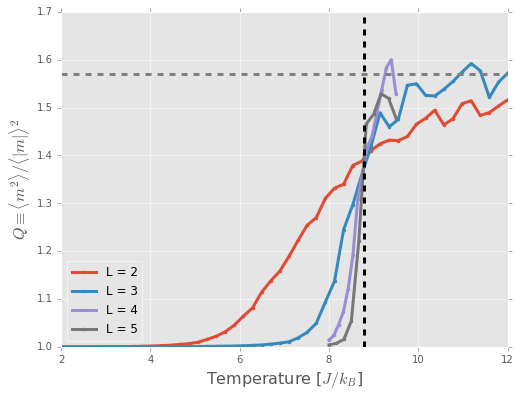
\includegraphics[width=\linewidth]{img/5D/binderQ}
    \end{minipage}
    \hspace{\fill} % note: no blank line here
    \begin{minipage}{0.47\textwidth}
    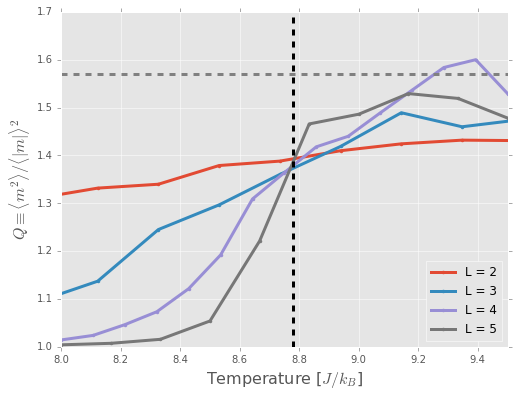
\includegraphics[width=\linewidth]{img/5D/binderQ_close}
    \end{minipage}
\caption{Five dimensions. Top row: Magnetization per spin (left) and specific heat (right). Middle row: susceptibility on linear (left) and semi-log (right) scales. Bottom row: Binder ratio $Q$ for the whole temperature sweep (left) and near $T_\text{c}$ (right). Dashed vertical line indicates critical temperature $T_{\text{c, 5D}}\approx1/0.11391498\approx8.7784767$ [Nuclear Physics B 895, 305-318 (2015)]. Dashed horizontal line in the Binder ratio figures indicates theoretical high-temperature limit of $Q=\pi/2$.}
\label{fig:5D_all}
\end{figure}
Figure~\ref{fig:5D_mag_loglog} shows the magnetization as a function of temperature on a log-log scale, along with a power law fit to the $L=4$ data, yielding a best-fit of $\beta=0.39612343$. The mean field value for $\beta$, which is exact in five dimensions is $\beta=1/(5-2)=1/3$, an error of $19\%$. Figure~\ref{fig:5D_corr} shows a log-log plot of correlation length $\xi$ as a function of temperature for $L=4$ and $L=5$. One could convince oneself that there is a peak in $\xi$ at $T_\text{c}$.
\begin{figure}[H]
   \centering
   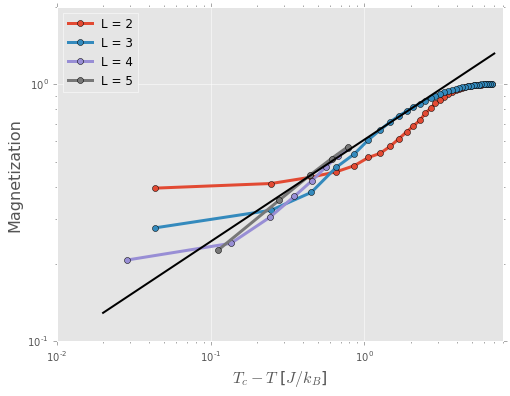
\includegraphics[width=0.6\textwidth]{img/5D/mag_loglog} % requires the graphicx package
   \caption{Log-log plot of the magnetization as a function of $T_\text{c}-T$ in five dimensions. Black line is a power law fit to the $L=4$ curve, yielding $\beta=0.39612343$.}
   \label{fig:5D_mag_loglog}
\end{figure}
\begin{figure}[H]
\centering
    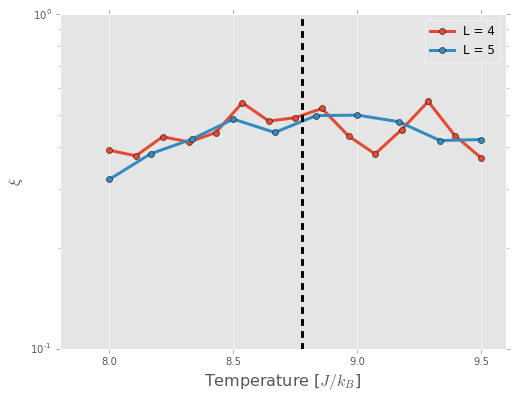
\includegraphics[width=0.6\textwidth]{img/5D/xi_T}
\caption{Semi-log plot of correlation length $\xi$ (extracted from a fit to an exponential $\sim e^{-r/\xi}$) as a function of temperature for $L=4,\,\&\,5$.}
\label{fig:5D_corr}
\end{figure}
Fitting $\chi_\text{max}(L)$ and $t_\text{max}(L)$ yields critical exponent estimates of $\gamma/\nu\approx2.789$, $\nu\approx0.328$, $\gamma\approx0.915$. The exact (mean field) values are $\nu=1/3$ and $\gamma=1$. This amounts to a 1.6\% error in $\nu$ and an $8.5\%$ error in $\gamma$. It appears we get a hint of mean field theory on small lattices in five dimensions.
\begin{figure}[H]
   \centering
   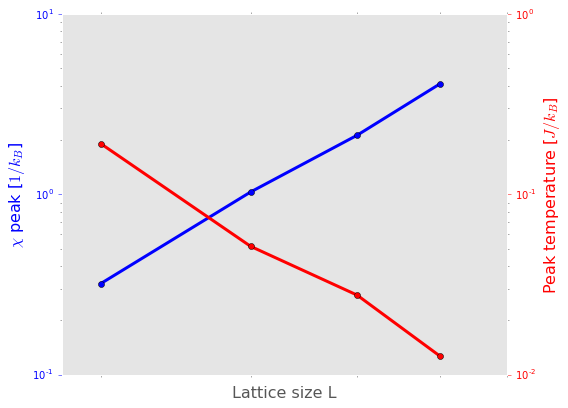
\includegraphics[width=0.6\textwidth]{img/5D/gam_nu} % requires the graphicx package
   \caption{Log-log plot of $\chi_\text{max}(L)$ and $t_\text{max}(L)$, yielding exponents of $\gamma/\nu\approx2.789$ and $\nu\approx0.328$.}
   \label{fig:5D_gam_nu}
\end{figure}
Given more time, I would simulate larger lattices with more temperatures near $T_\text{c}$ to try to get more reasonable values for the critical exponents.
%%%%%%%%%%%%%%%%%%%%%%%%%%%%%%%%%%%%%%%%%%%%%%%%%%%%
%
% Appendix
%
%%%%%%%%%%%%%%%%%%%%%%%%%%%%%%%%%%%%%%%%%%%%%%%%%%%%
\appendix
\section{Appendix}
\lstinputlisting[language=Python]{ising.py}
\end{document}